% !TEX root = ../monografia.tex
% !TeX spellcheck = pt_BR

% ----------------------------------------------------------
\chapter[Métodos de detecção de isquemia]{Métodos de detecção de isquemia}
\thispagestyle{empty}
\label{chap:chapter5}
% ----------------------------------------------------------

Neste capítulo serão introduzidos os métodos de detecção de isquemia selecionados para implementação. Antes de detalhar cada método nas seções \ref{sec:rocha}, \ref{sec:mohebbi} e \ref{sec:gopalak}, far-se-á na seção \ref{sec:methods} uma pequena discussão sobre as possíveis categorias de métodos existentes. Ao final do capítulo, um breve resumo é apresentado contendo os aspectos principais dos métodos estudados.

\section{Categorização de métodos}
\label{sec:methods}
Na literatura, os métodos para detecção de isquemia, assim como para detecção de outros tipos de doença cardíaca, empregam técnicas variadas de (i) processamento de sinais, (ii) extração de características e (iii) classificação das características. Cada um destes grupos corresponde a uma etapa do processamento, sendo que todas incluem técnicas amplamente diversificadas.

O primeiro grupo constitui o que se denomina etapa de \textbf{pré-processamento}. A tabela \ref{tab:preprocessing} mostra algumas categorias de técnicas desta etapa e referências de algoritmos em cada categoria. A tabela \ref{tab:extraction} agrupa alguns métodos de detecção de acordo com técnicas usadas na \textbf{extração}, enquanto a tabela \ref{tab:classification} agrupa-os de acordo com técnicas usadas na \textbf{classificação}. Contudo, as técnicas de análise para extração e classificação não se limitam às das tabelas apresentadas. Há ainda métodos que utilizam modelagem paramétrica, mineração de dados, autômatos finitos, métodos sintáticos, entre outras. Também é importante mencionar que muitos dos algoritmos referenciados na primeira tabela são incluídos como parte da etapa de pré-processamento dos métodos de detecção de isquemia, que por sua vez são referenciados nas demais tabelas.

\begin{table}[ht!]
    \centering
    \begin{tabular}{p{140pt}p{280pt}}
    \toprule
    Filtragem linear (FIR/IIR, suavização, diferenciação, etc.) &
    \cite{Chen2006, Elgendi2013, Okada1979, Pan1985, Daskalov1998}\\
    Filtragem adaptativa &
    \cite{Park1998}\\
    Interpolação polinomial &
    \cite{Badilini1991}\\
    Técnicas não-lineares (matemática morfológica, produtório, máximo/mínimo, etc.) &
    \cite{Chu1989, Okada1979, Sun2005, Suppappola1994, Trahanias1993, Pan1985}\\
    Decomposição wavelet &
    \cite{Chen2006, Park1998}\\
    Thresholding adaptativo &
    \cite{Chen2006, Elgendi2013, Sun2005, Pan1985}\\
    \bottomrule
\end{tabular}
    \caption[Categorias de métodos de acordo com as técnicas de pré-processamento]{Categorias de métodos de acordo com técnicas comuns de pré-processamento.}
    \label{tab:preprocessing}
\end{table}

\begin{table}[ht!]
    \centering
    \begin{tabular}{p{140pt}p{280pt}}
    \toprule
    Uso de template &
    \cite{Akselrod1987, Garcia2000, Couceiro2008, Mohebbi2007}\\
    Decomposição wavelet &
    \cite{Ranjith2003, Senhadji1995, Milosavljevic2006}\\
    Transform. ortogonal (PCA, Karhunen-Loève, Hermite) &
    \cite{Castells2007, Rocha2010, Afsar2007, Gopalakrishnan2004, Pang2005}\\
    Análise frequencial ou tempo-frequencial &
    \cite{Rocha2010, Senhadji1995, Badilini1992, Couceiro2008}\\
    Propriedades estatísticas (correlação, erro médio, etc.) &
    \cite{Ranjith2003, Badilini1992, Couceiro2008, Garcia2000}\\
    Conhecimento prévio &
    \cite{Elgendi2013, Papaloukas2000}\\
    Características pontuais (pontos J e isoelétrico, picos de ondas, desvio de segmento ST) &
    \cite{Akselrod1987, Goletsis2004, Papaloukas2000, Ranjith2003, Rocha2010, Senhadji1995, Vila1997, Badilini1992, Couceiro2008, Mohebbi2007}\\
    \bottomrule
\end{tabular}
    \caption[Categorias de métodos de acordo com as técnicas de extração]{Categorias de métodos de acordo com técnicas comuns de extração.}
    \label{tab:extraction}
\end{table}

\begin{table}[ht!]
    \centering
    \begin{tabular}{p{140pt}p{280pt}}
    \toprule
    Redes neurais artificiais &
    \cite{Papaloukas2001, Rocha2010, Afsar2007, Couceiro2008, Gopalakrishnan2004, Mohebbi2007, Pang2005, Stamkopoulos1997, Maglaveras1998}\\
    Fuzzy ou neuro-fuzzy &
    \cite{Exarchos2007, Vila1997}\\
    Conjunto de regras &
    \cite{Akselrod1987, Exarchos2006, Papaloukas2002}\\
    Clusterização &
    \cite{Badilini1992}\\
    Modelos de Markov &
    \cite{Andreao2004}\\
    Algoritmos genéticos &
    \cite{Goletsis2004}\\
    \bottomrule
\end{tabular}
    \caption[Categorias de métodos de acordo com as técnicas de classificação]{Categorias de métodos de acordo com técnicas comuns de classificação.}
    \label{tab:classification}
\end{table}


\section{Método de Rocha et al.}
\label{sec:rocha}
Este método é baseado em dois pontos-chave: (i) desvio do segmento ST com relação à linha de base e (ii) expansão do complexo QRS e da onda T em funções de Hermite. A figura \ref{fig:rochadiag} mostra o diagrama em blocos da estratégia adotada. As etapas do método são detalhadas a seguir.

\begin{figure}[ht]
    \centering
    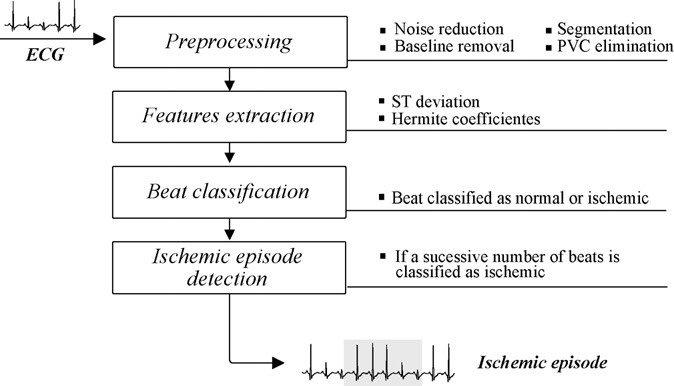
\includegraphics[width=300pt]{figures/chap5-rocha-diagram.png}
    \caption[Diagrama de blocos da estratégia utilizada no método de Rocha et al.]{Diagrama de blocos da estratégia proposta por Rocha et al. Extraído de \cite{Rocha2010}}
    \label{fig:rochadiag}
\end{figure}

\subsection*{Pré-processamento}
Nesta etapa, um sinal discreto contendo as amplitudes do ECG é processado com vistas à redução de ruído, segmentação em ondas características, eliminação de extra-sístoles ventriculares e, por último, remoção da linha de base.

A redução de ruído é realizada com um filtro passa-baixas de Butterworth de 4\textordfeminine{} ordem e frequência de corte 40 Hz. O sinal filtrado é então submetido a um procedimento de segmentação, em que as ondas características de cada batimento são identificadas. Na proposta dos autores, utiliza-se o algoritmo descrito em \cite{Sun2005}, baseado em derivação morfológica do sinal (um tipo de filtragem não linear, usando máximos e mínimos). Na saída obtêm-se as localizações de início, pico e fim de cada onda característica.

Após a segmentação, os batimentos passam por um procedimento de remoção de extra-sístole ventricular (ou PVC, do inglês \emph{premature ventricular contraction}), conforme descrito em \cite{Couceiro2008}. O último procedimento nesta etapa consiste em remover a linha de base em cada batimento cardíaco. Isto é necessário para as próximas etapas, onde se exige que os batimentos estejam bem alinhados com o nível isoelétrico do sinal.

\subsection*{Extração}
Nesta etapa, dois grupos de características são extraídos do ECG: (i) a medida do desvio de segmento ST e (ii) os coeficientes da expansão de Hermite do complexo QRS e das ondas T. Variações no desvio do segmento ST são usadas para discriminar os batimentos isquêmicos dos normais. De maneira similar, variações na morfologia do complexo QRS e da onda T indicam presença ou não de isquemia.

Para compor o primeiro grupo de características, dois valores são obtidos através de dois métodos distintos. Um deles é baseado na localização dos picos de onda R e na frequência cardíaca, conforme descrito em \cite{Pang2005}. O outro é derivado de uma análise do ECG em tempo-frequência, usando a transformada de Wigner-Ville descrita a seguir.

A distribuição de Wigner-Ville permite representar o espectro de frequências de um sinal contínuo ao longo do tempo. Ela é definida pela equação
\begin{equation}
    W_x(t,f) = \int_{-\infty}^{\infty} x\left( t+\frac{\tau}{2} \right) x^*\left( t-\frac{\tau}{2} \right) e^{-j2\pi f \tau} d\tau,
\end{equation}
onde o termo em $x$ é a função de autocorrelação instantânea e o operador $^*$ indica o conjugado complexo. Em tempo discreto, ela é chamada de pseudo-transformada de Wigner-Ville e assume a forma abaixo:
\begin{equation}
    W_x(nT,f) = 2T\sum_{p=-L_1}^{L_2} x[n+p]x^*[n-p]w[p]w^*[-p]e^{-j4\pi fp}.
    \label{equ:wigner}
\end{equation}

Nesta equação, $T$ é o período de amostragem e $w$ é uma janela simétrica de largura $L_1+L_2+1$. Os autores afirmam que o tamanho da janela deve ser maior que o do complexo QRS mais largo, para garantir que as características do formato de onda não sejam perdidas na transformação. Além disso, sabe-se que esta transformada pode ser calculada a partir da DFT (transformada discreta de Fourier) da autocorrelação de $x$ no tamanho da janela. Uma escolha conveniente para o tamanho da janela é uma potência de 2, pois neste caso o cálculo da DFT é mais eficiente. Por exemplo, assumindo que um complexo QRS não ultrapasse a largura de 100 ms e tomando uma frequência de amostragem de 250 Hz, pode-se utilizar uma janela de tamanho 32, pois $250\cdot 0,1 = 25$.

Após a transformação, soma-se os valores absolutos das componentes de baixa frequência do sinal em dois intervalos de tempo distintos: um à esquerda do pico de onda R e outro à direita do mesmo ponto. Os autores dizem utilizar os índices de frequência correspondentes a frequências entre 0 e 0,2 na escala normalizada. Entretanto, não mencionam quais os limites das faixas de tempo analisadas, nem mesmo o tipo de janela utilizado na Eq. \ref{equ:wigner}. Assume-se que a janela é do tipo retangular e que os limites das faixas de tempo devam ser estabelecidos conforme o caso.

O resultado da soma das componentes frequenciais provê informações sobre a concentração de energia nas duas faixas de tempo, sendo o restante do algoritmo uma simples busca pelo ponto mínimo em cada uma delas. O ponto mínimo à esquerda é o chamado ponto isoelétrico, enquanto o ponto mínimo à direita é chamado ponto J. Estes conceitos são discutidos em detalhe no artigo original. Basta apenas mencionar que a medida do desvio de segmento ST é a diferença entre as amplitudes nos pontos J e isoelétrico.

Para o segundo grupo de características, os autores propuseram uma técnica baseada na expansão em funções de Hermite. Já foi vista no capítulo \ref{chap:chapter3} a definição dessas funções em tempo contínuo para o caso particular em que elas não apresentam um parâmetro de dilatação. Aqui será reintroduzida a expressão da função de Hermite de tempo contínuo para o caso dilatado por um fator $l$, e usando a notação em $t$ da variável independente:
\begin{equation}
    \psi_n(t,l) = \left(\frac{e^{-(t/l)^2}}{n!2^n\sqrt{\pi}}\right)^\frac{1}{2} H_n\left(\frac{t}{l}\right)
\end{equation}

Pode-se perceber que aqui os autores optam por uma representação em tempo contínuo. A expansão consiste em obter uma lista de coeficientes que satisfazem a equação
\begin{equation}
   \hat{y}(t) = \sum_{j=0}^{M-1} c_j\psi_j(t,l),
\end{equation}
onde $c_j$ é o coeficiente da $j$-ésima função de Hermite e $M$ é o número de funções utilizadas na aproximação. Os coeficientes são dados pela solução algébrica do problema de minimização do erro quadrático, conforme a equação
\begin{equation}
    C = (H^TH)^{-1}H^TY,
\end{equation}
onde $C$ é um vetor coluna contendo os $M$ coeficientes da expansão, $Y$ é um vetor coluna contendo as amplitudes do sinal original e $H$ é uma matriz cujas colunas são as funções de Hermite:
\begin{equation}
    H = [\psi_0\ \psi_1\ \cdots\ \psi_{m-1}].
\end{equation}

Antes deste procedimento, contudo, o sinal de um batimento cardíaco é separado em dois segmentos: um deles contendo as amostras do complexo QRS e o outro, as da onda T. Essa separação permite aproximar melhor o formato do batimento em cada região, já que o complexo QRS e a onda T possuem morfologia distinta. Além disso, essas ondas estão bastante afastadas temporalmente, o que indica a necessidade de muitas funções de Hermite na aproximação caso se queira aproximar o sinal do batimento na íntegra. Os autores, pelo contrário, sugerem a utilização de apenas 6 funções na aproximação e, portanto, se justifica a separação em dois segmentos.

Os autores ainda mencionam a necessidade de reamostrar cada segmento para 64 amostras, afim de utilizar sempre a mesma largura para as funções de Hermite. Isto significa que a matriz $H$ pode ser calculada previamente e não se modifica durante a execução do algoritmo, permitindo aumento de eficiência na computação. Assim, dois conjuntos de 64 amostras por batimento são submetidos ao procedimento de expansão de Hermite, obtendo-se como resultado duas listas de 6 coeficientes. Estas listas são então incorporadas ao conjunto de características, de cuja parte já fazem as medidas do desvio de segmento ST.

\subsection*{Classificação}
O esquema de classificação usado por Rocha et al. envolve o uso de redes neurais artificiais. Para cada derivação de ECG, duas redes do tipo \emph{feed-forward} são treinadas com as características obtidas na etapa de extração. O algoritmo utilizado no treinamento é o Levenberg-Marquardt. O número de camadas é o mesmo para todas as derivações, sendo duas camadas ocultas mais a de entrada e a de saída. A função de transferência é a tangente sigmóide. O número de neurônios na entrada corresponde ao número de características extraídas, qual seja, $2+6+6=14$, enquanto a saída conterá apenas um neurônio, que fornece o resultado correspondente a elevação ou a depressão do segmento ST. O critério de inversão da onda T não é utilizado nesta estratégia. A figura \ref{fig:rochaclass} ilustra o esquema de classificação assim proposto.

\begin{figure}[ht]
    \centering
    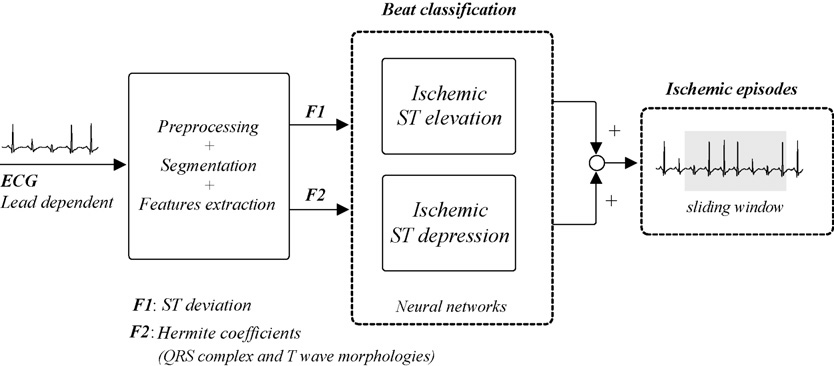
\includegraphics[width=400pt]{figures/chap5-rocha-class.png}
    \caption[Diagrama da estratégia de classificação de Rocha et al.]{Diagrama da estratégia de classificação de Rocha et al. Extraído de \cite{Rocha2010}}
    \label{fig:rochaclass}
\end{figure}

Ainda nesta etapa, há um procedimento de detecção de episódios isquêmicos. Sugerem os autores que um episódio isquêmico seja detectado toda vez que uma sequência de 40 batimentos tiver pelo menos metade classificada como isquêmica. Assim, uma janela de tamanho 40 percorre o resultado da classificação avançando um batimento por vez e sinaliza a ocorrência de um episódio quando o número de batimentos isquêmicos ultrapassa 20, ou sinaliza a ausência de episódio quando este número cai a 20 ou menos. Num segundo passo, episódios adjacentes com separação menor que 40 batimentos são unidos.


\section{Método de Mohebbi e Moghadam}
\label{sec:mohebbi}
Este método tem como principal recurso a obtenção de um modelo (ou \emph{template}, em inglês) de batimento cardíaco considerado normal, extraído do próprio registro sobre o qual se deseja fazer a detecção de isquemia. As etapas do algoritmo podem ser visualizadas no diagrama da figura \ref{fig:mohebbidiag} e seus detalhes são discutidos a seguir.

\begin{figure}[ht]
    \centering
    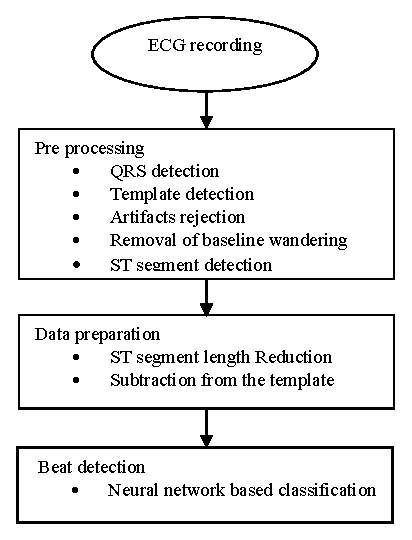
\includegraphics[width=250pt]{figures/chap5-mohebbi-diagram.pdf}
    \caption[Diagrama de blocos da estratégia proposta por Mohebbi e Moghadam]{Diagrama de blocos da estratégia proposta por Mohebbi e Moghadam. Extraído de \cite{Mohebbi2007}}
    \label{fig:mohebbidiag}
\end{figure}

\subsection*{Pré-processamento}
Esta etapa consiste de identificação dos complexos QRS, obtenção de um modelo de batimento, remoção de ruído, rejeição de artefatos e extração do segmento ST. A identificação dos complexos QRS e dos picos de onda R é feita através de um algoritmo descrito em \cite{Tompkins1993}, que faz uso extensivo de filtragem para realçar os complexos QRS e de \emph{thresholding} para a detecção. Na saída obtêm-se uma lista com as localizações dos picos de onda R.

Em seguida, os primeiros 30 segundos do registro de ECG são inspecionados afim de detectar artefatos ou batimentos considerados anômalos. Tal procedimento é feito através de uma estimativa do ponto isoelétrico e do ponto J de cada batimento. A estimativa se dá pela análise do gradiente do sinal. Caso nenhum dos dois pontos seja detectado, o batimento em questão é considerado como artefato e removido da lista. Os batimentos remanescentes são usados para construção do modelo, que é a média aritmética entre as amplitudes dos batimentos. Em seguida, o resto do sinal é processado e a linha de base é estimada através de interpolação \emph{spline} cúbica, segundo o método descrito em \cite{Badilini1991}.

\subsection*{Extração}
Na etapa de extração, detecta-se o ponto J de cada batimento usando novamente o gradiente do sinal. Neste caso, uma janela de 100 ms à direita do pico de onda R é suavizada por um filtro de média móvel. Em seguida, busca-se na janela o primeiro intervalo de 20 ms cujo declive médio seja menor que 2,5 mV/s em valor absoluto. Toma-se o ponto central deste intervalo como o ponto J. Obtidos os pontos J, assume-se que os segmentos ST iniciem neste ponto e possuam largura pré-definida de 160 ms. O mesmo se aplica ao batimento modelo, do qual se extrai o segmento ST usado como referência no algoritmo.

Os dados que constituem a entrada para a etapa de classificação são a diferença entre o segmento ST dos batimentos e o segmento ST de referência. Dada uma taxa de amostragem $f_s$, o segmento ST possui $\lfloor0.16f_s\rfloor$ amostras. Afim de reduzir o tamanho do conjunto de características, os sinais de segmento ST (inclusive o do modelo) são reamostrados para 20 amostras.

\subsection*{Classificação}
Mohebbi e Moghadam também fazem uso de redes neurais artificiais para a etapa de classificação. Aqui, uma única rede neural é treinada usando o algoritmo de \emph{backpropagation} com taxa de aprendizado adaptativa, combinado ainda com a técnica de treinamento com \emph{momentum}. Os autores justificam o uso dessas técnicas argumentando que o desempenho do \emph{backpropagation} é bastante sensível ao valor estabelecido para a taxa de aprendizagem, sendo que o valor ótimo deste parâmetro varia de acordo com a complexidade da superfície do erro. Dessa forma, uma taxa de aprendizado adaptativa se manterá no maior valor possível enquanto também permanece estável. O treinamento com \emph{momentum} significa que a rede responderá não apenas ao gradiente local, mas também a tendências recentes na superfície do erro.

A camada de entrada da rede possui 20 neurônios, que recebem a sequência de valores oriunda da etapa de extração. A rede possui uma camada oculta também com 20 neurônios. A camada de saída contém dois neurônios, cujo valor de saída está no intervalo real de 0 a 1. As saídas da rede neural são o grau de pertinência a cada uma das classes (presença ou ausência de isquemia), sendo que o máximo entre as duas designa a classificação final. O treinamento da rede se encerra quando a soma do erro quadrático for menor que 0,01 ou quando o número limite de 2000 épocas é atingido.


\section{Método de Gopalakrishnan et al.}
\label{sec:gopalak}

O terceiro e último método estudado faz uso de uma série de propriedades da álgebra linear e também da relação entre as funções discretas de Hermite e a matriz de Fourier\footnote{matriz de Fourier é aquela que, multiplicada por um vetor, resulta na DFT do vetor}. As etapas do algoritmo são ilustradas pelo diagrama da figura \ref{fig:gopalakdiag}, sendo detalhada a seguir.

\begin{figure}[ht]
    \centering
    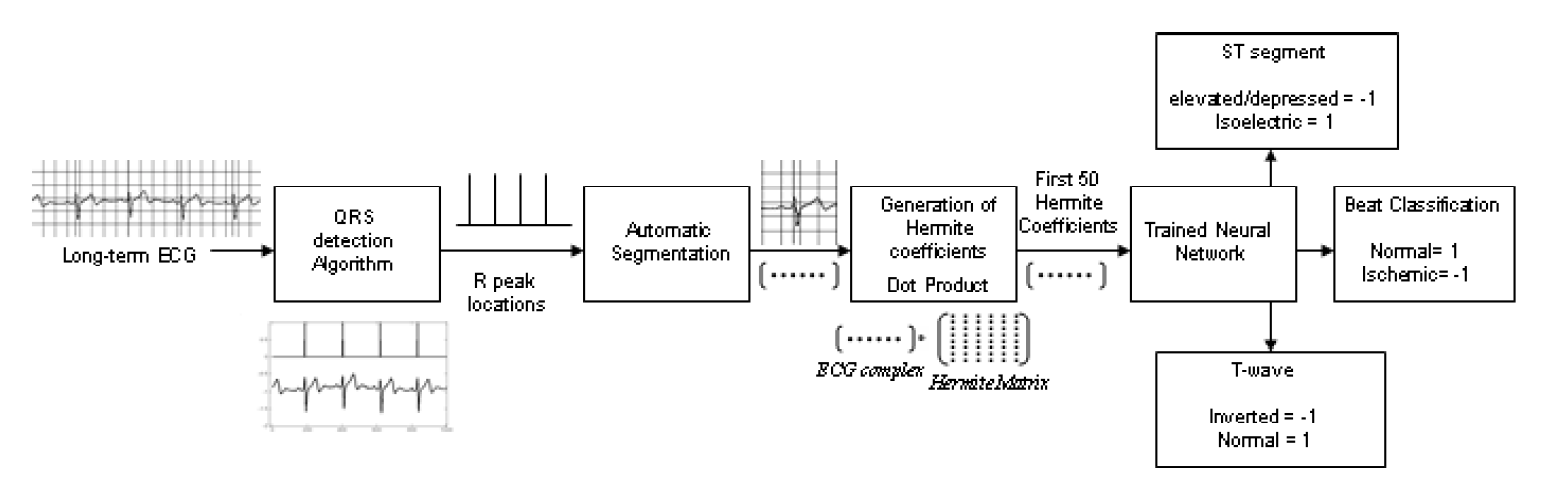
\includegraphics[width=1.0\textwidth]{figures/chap5-gopalak-diagram.png}
    \caption[Diagrama de blocos da estratégia adotada por Gopalakrishnan et al.]{Diagrama de blocos da estratégia adotada por Gopalakrishnan et al. Extraído de \cite{Gopalakrishnan2004}}
    \label{fig:gopalakdiag}
\end{figure}

\subsection*{Pré-processamento}
O método proposto não inclui nenhuma informação especial sobre procedimentos na etapa de pré-processamento, com exceção da própria detecção de batimentos cardíacos. Neste caso, os autores utilizam o mesmo algoritmo de detecção QRS mencionado para o caso do método anterior, qual seja, o algoritmo de Tompkins. Após obtenção dos picos de onda R, cada batimento deve ser centralizado neste ponto e sua largura é equivalente ao intervalo entre o seu pico e o do batimento vizinho (chamado intervalo R-R, ou apenas RR). Entretanto, técnicas como as de remoção da linha de base ou redução de ruído/interferência não estão presentes neste método.

\subsection*{Extração}
Para cada batimento, os primeiros 50 coeficientes de Hermite são extraídos, utilizando exatamente o mesmo ferramental introduzido no capítulo \ref{chap:chapter3}, no que diz respeito às funções discretas de Hermite. Estes coeficientes constituem, integralmente, o conjunto de características fornecido à etapa de classificação. Os autores ainda explicam, baseando-se em trabalhos passados e também pela observação do erro RMS (do inglês, \emph{root mean square}) percentual, que o uso de 50 coeficientes e de um parâmetro de dilatação $b=1$, garantem uma aproximação bastante boa.

\subsection*{Classificação}
Gopalakrishnan et al. utilizaram cinco redes neurais em seu esquema de classificação. A justificativa é que o resultado de redes individuais pode variar em casos limítrofes de isquemia. Desse modo, o resultado majoritário de um comitê de cinco redes fornece a decisão final sobre a classe a que pertence um batimento. As redes possuem três camadas ocultas com diferentes números de neurônios em cada uma. A camada de saída possui dois neurônios, que indicam presença ou não de alterações no segmento ST e presença ou não de inversão da onda T.

Os autores não especificam um algoritmo para o treinamento das redes. Contudo, relatam a realização de um procedimento adicional em cada registro de ECG de longa duração. Eles explicam que as redes são retreinadas usando alguns exemplares de ciclo cardíaco normal do ECG e argumentam que isso fornece às redes um ``toque'' das características normais de segmento ST e onda T daquele registro em particular.


\section{Resumo}
Neste capítulo foram apresentados os métodos de detecção de isquemia estudados no trabalho. Primeiramente, algumas categorias foram usadas para agrupar os métodos de acordo com as principais técnicas de detecção utilizadas.

Depois, foi visto em detalhe o método proposto por Rocha et al., que emprega um procedimento sofisticado de segmentação de batimentos e também várias técnicas para eliminação de ruído, linha de base e extra-sístoles ventriculares (PVCs). O método sugere a utilização de dois grupos de características: o do desvio de segmento ST e o dos coeficientes da expansão em funções de Hermite. Particularmente, este método faz uso de análise espectral dos batimentos para obtenção do ponto J. Na etapa de classificação, cada derivação tem uma rede neural treinada somente com características advindas daquela derivação. As características usadas no treinamento das redes são a elevação e a depressão do segmento ST.

O método de Mohebbi et al., embora um pouco menos sofisticado, também emprega diversas técnicas de pré-processamento para remover a linha de base, detectar os pontos J e isoelétrico e eliminar artefatos. Em especial, este método constrói um modelo de batimento cardíaco e de segmento ST, do qual se obtém a diferença com os demais segmentos ST extraídos. A etapa de classificação deste método é bastante simples, já que emprega apenas uma rede neural para todas as derivações. Aqui também são usadas a elevação e a depressão do segmento ST no treinamento.

Por fim, foi apresentado o método proposto por Gopalakrishnan et al. Este poderia ser considerado o mais simples dos três, já que não faz uso de nenhuma técnica especial na etapa de pré-processamento. Sua etapa de extração também é simples, pois se resume a um produto matricial correspondendo à expansão em funções discretas de Hermite. A etapa de classificação do método emprega cinco redes neurais, sem que haja distinção entre as derivações, e computa o resultado como a decisão majoritária das cinco redes. Todas as características indicativas de isquemia são usadas no treinamento das redes deste método.
